\section{interaction overview diagrams}

\subsection{Introduction}

Nous avons réalisé nos interaction overview diagrams sur base de nos use cases diagrams. 
Ce qui nous a permis de détailler la structure de ces diagrammes intuitivement.
\newline

\begin{flushleft}
Ces derniers permettront d’obtenir une idée globale du parcours des utilisateurs sur l’application ainsi que les fonctionnalités leur étant disponibles.
\end{flushleft}
\newline
\newline

\begin{flushleft}
Nous décrirons donc deux applications, l’application « client » et l’application « fournisseur » et de nouveau, nous verrons apparaître des points communs entre ces dernières.
\end{flushleft}

\newpage
\subsection{Points communs}

\begin{enumerate}[1.]
\item  \textbf{Système de logs}: 

\newline
Une fois que l’utilisateur arrivera sur l’application, plusieurs choix s’offriront à lui. Soit ce dernier est nouveau et il peut donc s’enregistrer en respectant les conditions qui lui sont imposées telles qu’une adresse mail valide, vérifiée par une demande de confirmation, et inexistante sur l’application, la mention de son rôle sur l’application (client ou fournisseur), un mot de passe ayant un niveau de sécurité convenable et le choix de sa langue, soit, il possède déjà un compte et se connecte. 
\newline
Cependant, celui-ci pourra réinitialiser son mot de passe à l’aide d’un mail de confirmation ou réessayer de se connecter si lors de la vérification des données, les identifiants sont invalides.
\newline
De plus, lorsque l’utilisateur sera connecté sur l’application, il aura la possibilité de se déconnecter s’il le souhaite.

\newline
\newline

\item \textbf{Menu représenté par un « grand » fork :}

\newline
Une fois connecté, l’utilisateur aura accès à un menu reprenant la déconnexion, l’accès aux paramètres, les notifications et les éléments lui étant propres en fonction qu’il soit fournisseur ou client. 
Cette façon de penser nous semblait suffisamment intuitive pour que l’utilisateur puisse naviguer sur l’application facilement. 
Nous avons également choisi de permettre un « retour » à ce menu lorsque nous sommes dans les sections le composant.

\newline
\newline

\item \textbf{Accès aux paramètres :}
\newline
Une fois sur l’onglet des paramètres, plusieurs choix s’offrent à lui : 

\begin{enumerate}[a)]
\newline
\item Gérer les langues : plus précisément, il pourra en ajouter, en choisir une qui sera sa langue favorite et de changer la langue actuelle de l'application comme expliqué précédemment dans les Use cases diagrams.

\newline
\item Modifier son mot de passe : pour ce faire, l’utilisateur recevra un mail de confirmation permettant de le changer en toute sécurité.
\end{enumerate}

\item \textbf{Les notifications :}
\newline
Une fois sur cette section, l’utilisateur pourra répondre à ses notifications, c’est-à-dire, marquer comme lues les contrats, les accepter, les refuser ou encore de voir leurs détails à savoir les données relatives à ces derniers. 
\newline
De surcroît, s’il le désire, ce dernier aura le droit de rafraichir ses notifications par lui-même sans attendre que cela se réalise automatiquement.

\end{enumerate}

\newpage
\subsection{Accès à l'application pour les clients}

Lorsque d’un client voudra \textbf{voir ses portefeuilles}, \newline il retrouvera plusieurs fonctionnalités :

\begin{enumerate}[1.]
\item Créer un portefeuille
\item Fermer un portefeuille
\item Visualisation des données de consommation
\item Gérer les données
\end{enumerate}

\[
\\[1mm]
\]

\begin{enumerate}[-]
\item \textbf{Créer un portefeuille : }
\newline
Cette première option permettra au client comme son nom l’indique de créer un portefeuille. 
\newline
Dans cette optique, il devra rentrer le nom et l’adresse du portefeuille, le code EAN et ajouter les contrats liés.

\item \textbf{Fermer un portefeuille :}
\newline
Cela donnera la possibilité au client de clôturer un portefeuille, une fois qu’il n’en aura plus d’utilité.

\item \textbf{Visualisation des données de consommation :}
\newline
Le client pourra observer les valeurs associées à sa consommation, ainsi que les contrats étant liés à ces dernières.

\item \textbf{Gérer les données :} 
\newline
Il sera également apte à les modifier, c’est-à-dire, renouveler ses données de consommation et ajouter, modifier ou supprimer les contrats étant associés à un portefeuille.
\newline Grâce à cette option, ce dernier aura pleinement la main sur ses portefeuilles et aura la faculté de les reformer à sa guise.
\end{enumerate}

\newpage

\begin{flushleft}
Le menu offre en outre la possibilité de \textbf{voir les contrats} ou plus précisément de voir ses contrats, l’utilisateur sera donc en mesure de, d’ :
\end{flushleft}
\begin{enumerate}[1.]
\item Ajouter des contrats
\item Fermer des contrats
\end{enumerate}

\[
\\[1mm]
\]

\begin{enumerate}[-]
\item \textbf{Ajouter des contrats :}
\newline
Le client se retrouvera alors sur la page des \textbf{fournisseurs et contrats relatifs} répertoriant tous les contrats qu’il ne possède pas encore et les verra en plus amples détails avant de les ajouter s’il le désire.

\item \textbf{Fermer des contrats :}
\newline
Cela lui donnera la possibilité de clôturer un contrat s’il trouve cela plus judicieux.

\newline
\newline

L’ajout et la fermeture de contrats impliquera une \textbf{notification} sur l’application du fournisseur en question.
\newline
Nous avons décidé de laisser la possibilité au client de voir les fournisseurs et contrats relatifs sans forcément passer par la liste de ses contrats afin de lui permettre un accès plus rapide.
\end{enumerate}

\newpage

\begin{figure}[h]
\centering
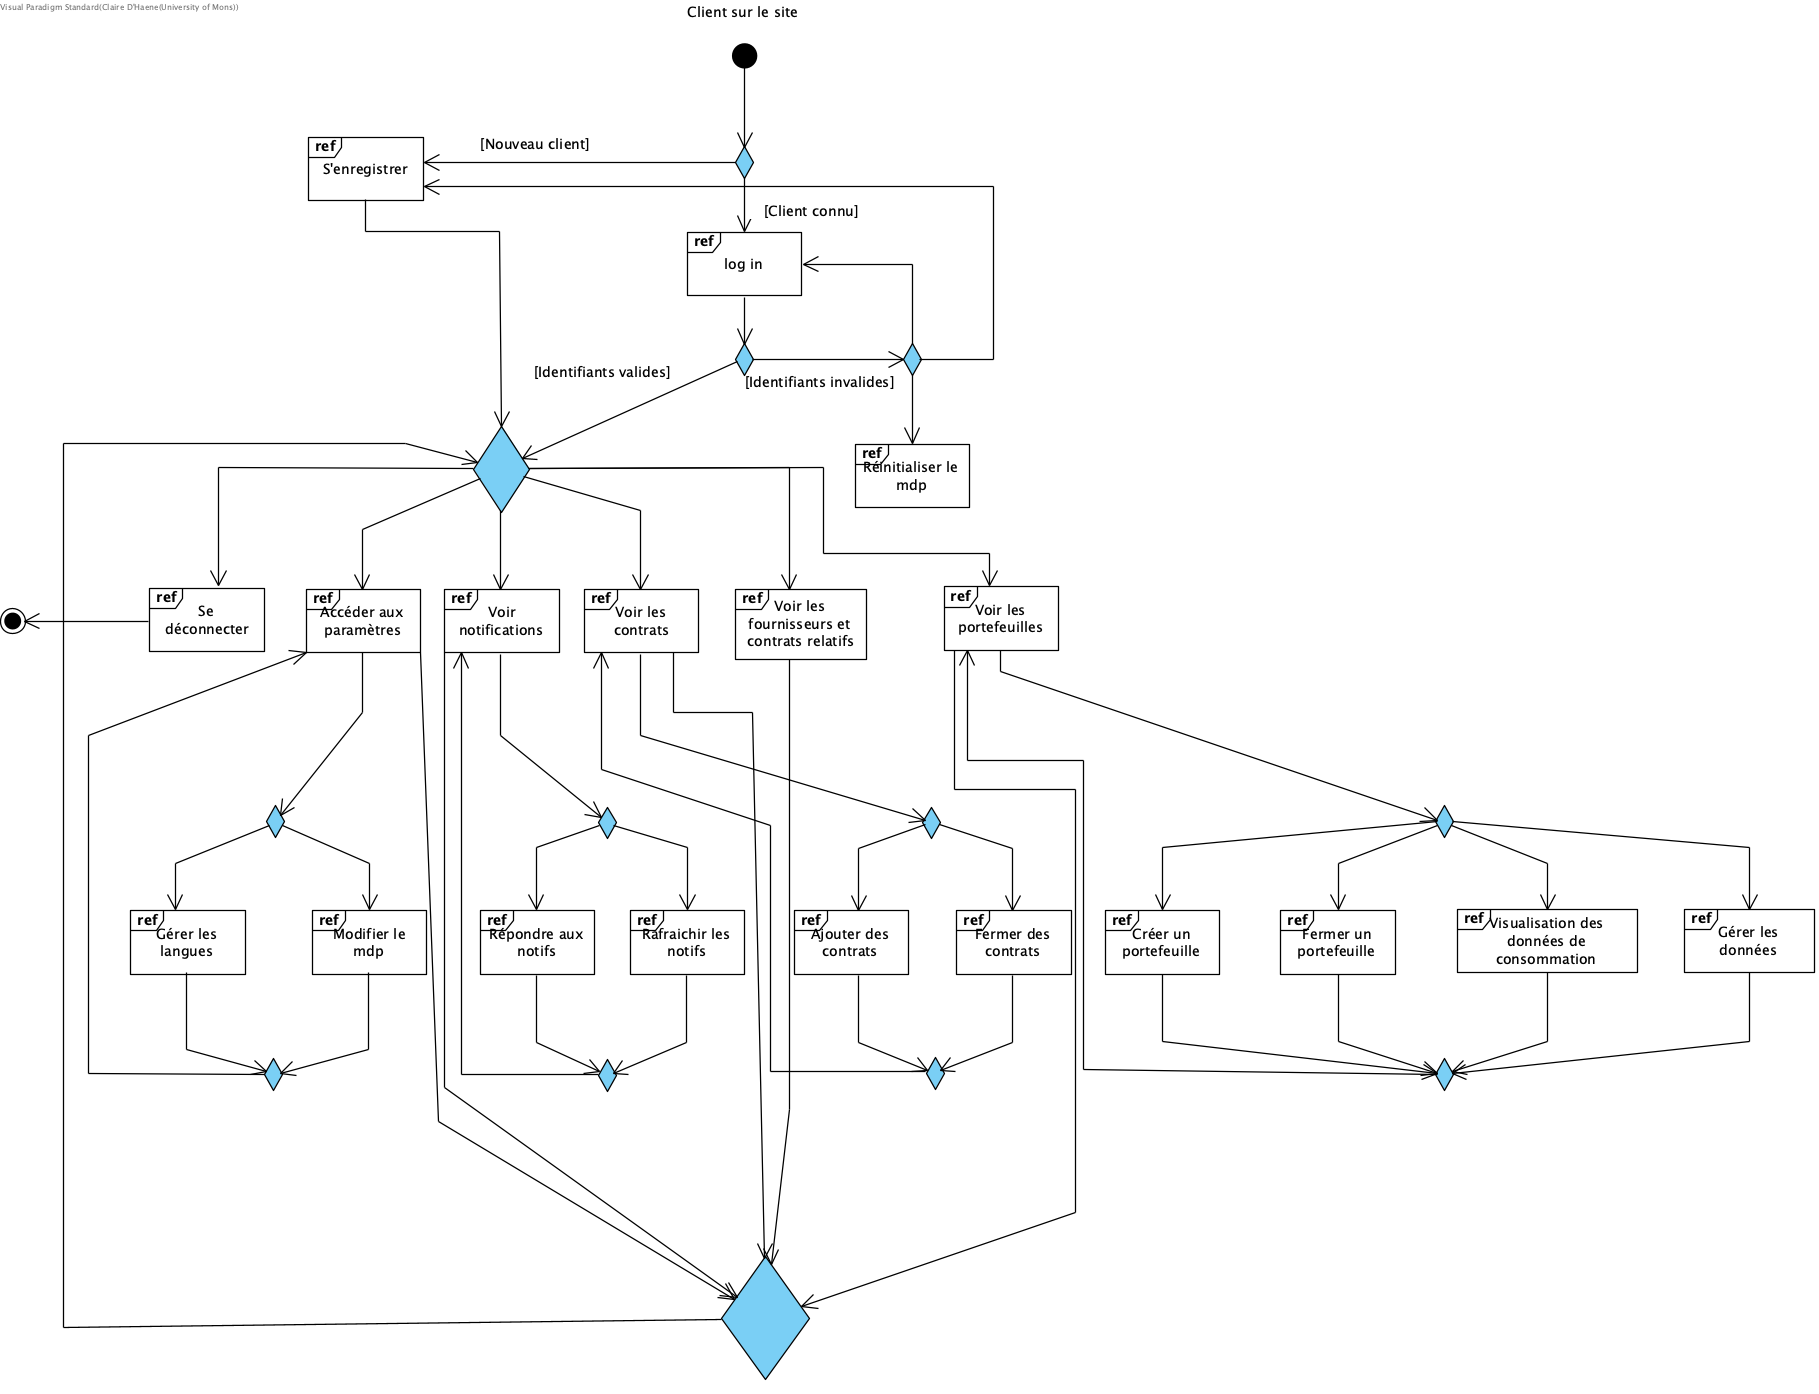
\includegraphics[width = 1\textwidth]{overview/overview-client.png}
\end{figure}

\newpage

\subsection{Accès à l'application pour les fournisseurs}

Au moment où le fournisseur accèdera à l’onglet \newline « \textbf{Voir les contrats clients} », plusieurs choix s’offriront à lui :
\begin{enumerate}[1.]
\item Ajouter des contrats
\item Fermer des contrats
\item Changer les paramètres des contrats
\end{enumerate}

\[
\\[1mm]
\]

\begin{enumerate}[-]
\item \textbf{Ajouter des contrats :} 
\newline
Cette option permettra au fournisseur d’ajouter de nouveaux contrats qu’il aura créés aux contrats déjà existants en spécifiant les valeurs leur relatives (prix, type de fourniture et compteurs).


\item \textbf{Fermer des contrats : }
\newline
Cela lui donnera la possibilité de clôturer un contrat, une fois qu’il n’en aura plus d’utilité.

\item \textbf{Changer des contrats : }
\newline
Le fournisseur sera apte à changer les termes du contrat s’il trouve cela approprié.
\newline Évidemment comme pour la fermeture de contrats, le changement sera notifié au client.
\end{enumerate}

\newpage
\begin{flushleft}
De plus, le fournisseur sera à même de « \textbf{Voir ses clients} » de manière distincte, plus précisément, ce dernier retrouvera une liste de ses clients avec les contrats leur étant associés :
\end{flushleft}
\begin{enumerate}[1.]
\item Ajouter un client
\item Supprimer un client
\item Voir les données de ses clients
\item Gérer les données de ses clients
\end{enumerate}

\[
\\[1mm]
\]

\begin{enumerate}[-]

\item \textbf{Ajouter un client : }
\newline
Ce dernier aura la capacité d’ajouter un client en l’associant à un de ses contrats en particulier.

\item \textbf{Supprimer un client :}
\newline
Cela donnera la possibilité au fournisseur de clôturer tous les contrats actifs avec un client, s’il est d’avis que cela est nécessaire.

\item \textbf{Visualisation des données de ses clients :}
\newline
Celui-ci pourra observer les valeurs associées aux contrats de ses clients, ainsi que leur consommation.

\item \textbf{Gérer les données de ses clients : }
\newline
Le fournisseur aura également la capacité de les modifier, c’est-à-dire, modifier, ajouter ou supprimer les contrats étant associés à un client.
\newline
Grâce à cette option, ce dernier aura pleinement la main sur ses clients et aura la faculté de les gérer à sa guise.
\newline
L’ajout, la modification et la fermeture de contrats impliquera une notification sur l’application du client en question.

\end{enumerate}

\newpage

\begin{figure}[h]
\centering
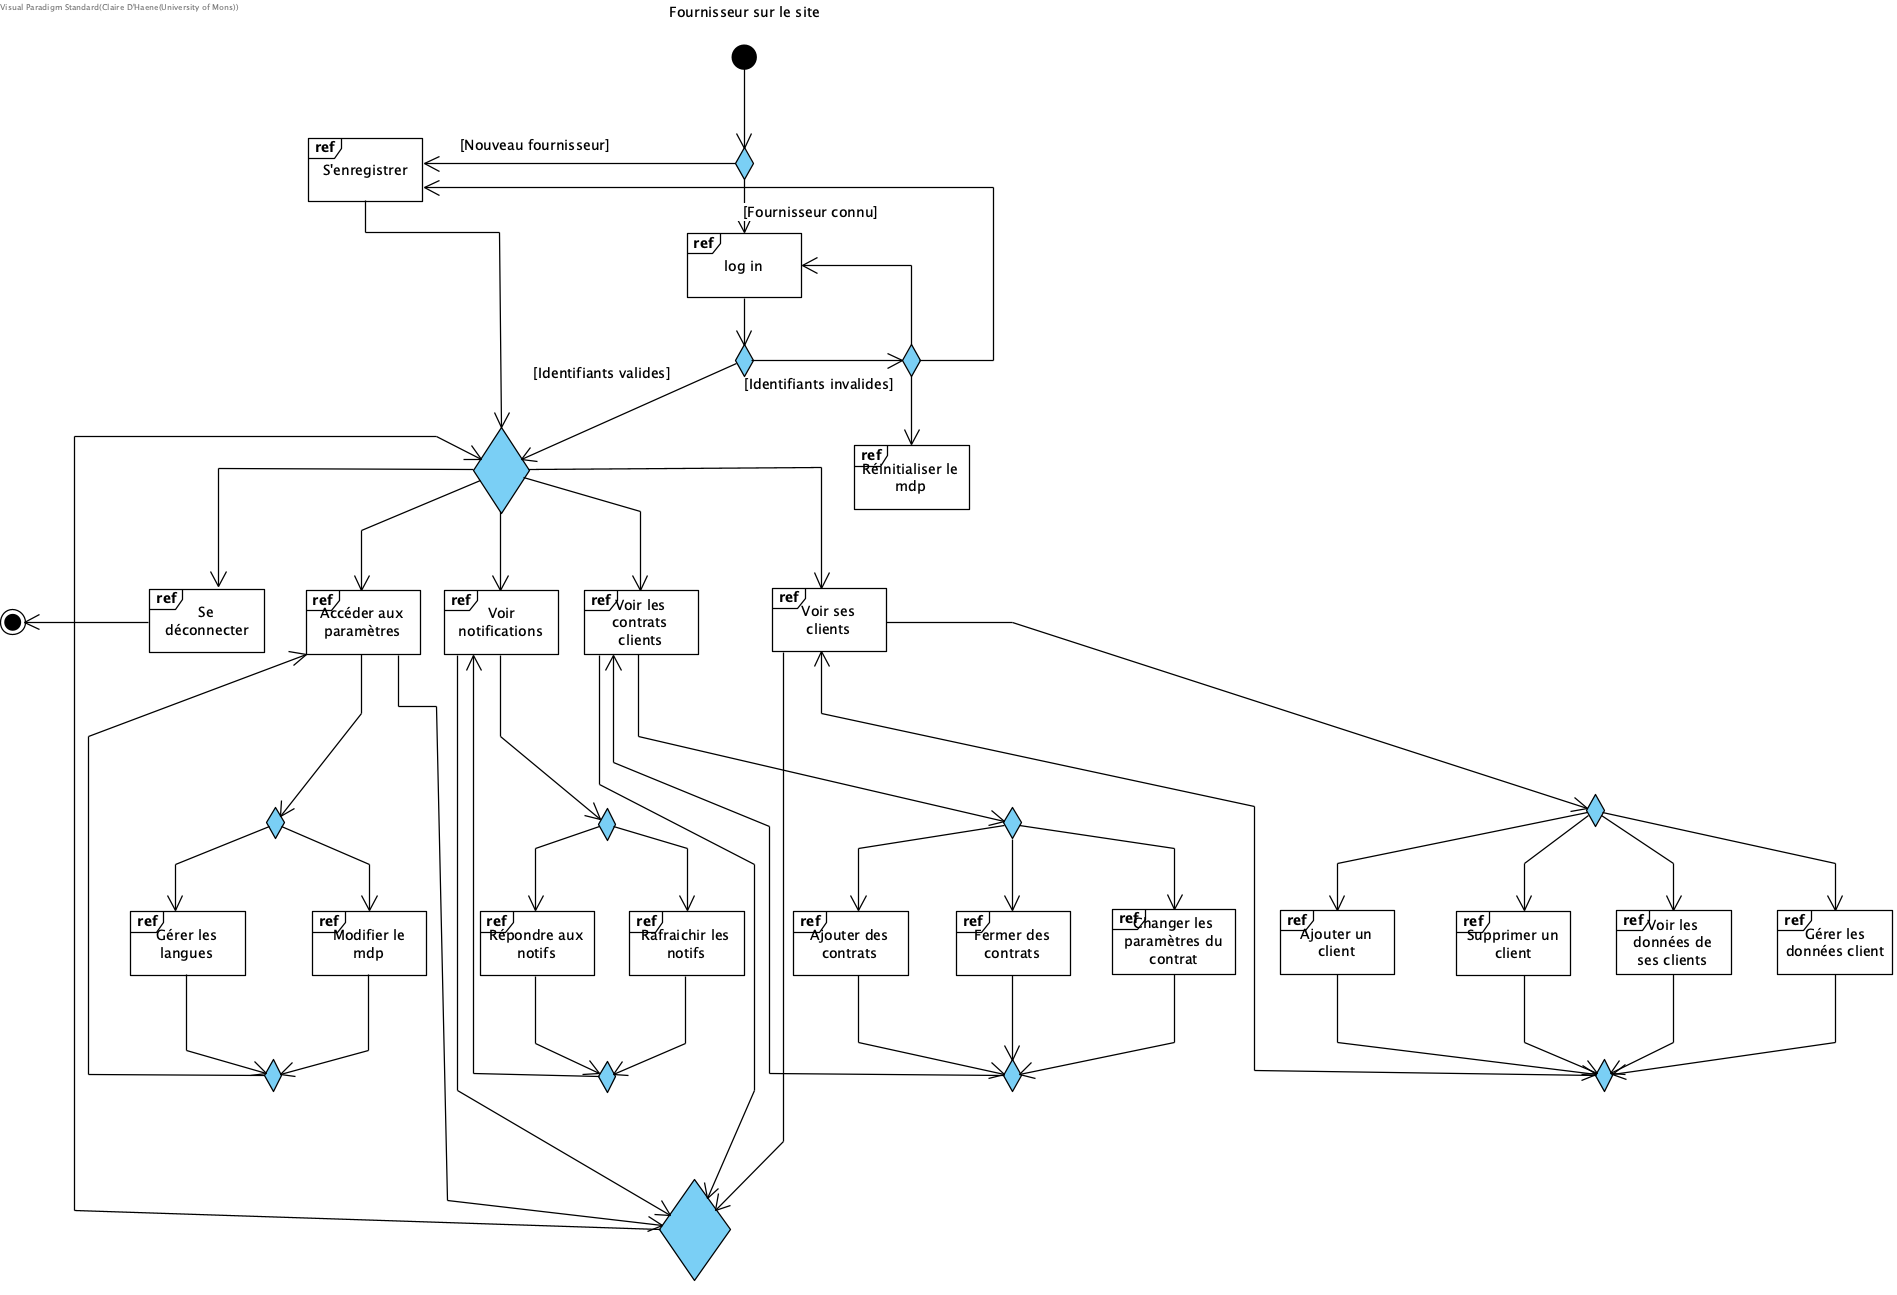
\includegraphics[width = 1\textwidth]{overview/overview-fournisseur.png}
\end{figure}